模板技术有时会导致类模板具有许多不同的模板类型参数,这些参数中的许多都有合理的默认值。定义此类类模板的方法如下:

\begin{lstlisting}[style=styleCXX]
template<typename Policy1 = DefaultPolicy1,
		typename Policy2 = DefaultPolicy2,
		typename Policy3 = DefaultPolicy3,
		typename Policy4 = DefaultPolicy4>
class BreadSlicer {
	...
};
\end{lstlisting}

这样的模板通常可以使用BreadSlicer<>语法与默认模板参数值一起使用,若必须指定非默认参数,那么前面的参数也必须指定(即使可能有默认值)。

显然,若能够使用类似于BreadSlicer<Policy3 = Custom>的构造,而不是使用BreadSlicer<DefaultPolicy1, DefaultPolicy2, Custom>的构造,将会更有吸引力。接下来,我们开发了一种技术来实现这一点。

\begin{tcolorbox}[colback=webgreen!5!white,colframe=webgreen!75!black]
\hspace*{0.75cm}注意,类似的函数调用参数的语言扩展在C++标准化过程中提出过(但被拒绝)(详见第17.4节)。
\end{tcolorbox}

技术包括将默认类型值放在基类中,并通过派生进行重写。通过辅助类提供类型参数,而不是直接指定类型参数,可以使用BreadSlicer<Policy3\_is<Custom>{}>。因为每个模板参数可以描述任何策略,默认值相同。换句话说,每个模板参数都等价:

\begin{lstlisting}[style=styleCXX]
template<typename PolicySetter1 = DefaultPolicyArgs,
		typename PolicySetter2 = DefaultPolicyArgs,
		typename PolicySetter3 = DefaultPolicyArgs,
		typename PolicySetter4 = DefaultPolicyArgs>
class BreadSlicer {
	using Policies = PolicySelector<PolicySetter1, PolicySetter2,
									PolicySetter3, PolicySetter4>;
	// use Policies::P1, Policies::P2, ... to refer to the various policies
	...
};
\end{lstlisting}

剩下的挑战是编写PolicySelector模板,必须将不同的模板参数合并为一个类型,该类型用指定的非默认值覆盖默认类型别名成员。这种合并可以通过继承实现:

\begin{lstlisting}[style=styleCXX]
// PolicySelector<A,B,C,D> creates A,B,C,D as base classes
// Discriminator<> allows having even the same base class more than once
template<typename Base, int D>
class Discriminator : public Base {
};

template<typename Setter1, typename Setter2,
		typename Setter3, typename Setter4>
class PolicySelector : public Discriminator<Setter1,1>,
						public Discriminator<Setter2,2>,
						public Discriminator<Setter3,3>,
						public Discriminator<Setter4,4> {
};
\end{lstlisting}

注意中间Discriminator模板的使用,需要允许各种Setter是相同的类型。(同一类型不能有多个直接基类。另一方面,间接基类可以具有与其他基类相同的类型。)

如前所述,可以在基类中收集默认值:

\begin{lstlisting}[style=styleCXX]
// name default policies as P1, P2, P3, P4
class DefaultPolicies {
	public:
	using P1 = DefaultPolicy1;
	using P2 = DefaultPolicy2;
	using P3 = DefaultPolicy3;
	using P4 = DefaultPolicy4;
};
\end{lstlisting}

若多次继承这个基类,则必须小心避免歧义。因此,需要确保基类是虚继承的:

\begin{lstlisting}[style=styleCXX]
// class to define a use of the default policy values
// avoids ambiguities if we derive from DefaultPolicies more than once
class DefaultPolicyArgs : virtual public DefaultPolicies {
};
\end{lstlisting}

最后,还需要一些模板来覆盖默认策略值:

\begin{lstlisting}[style=styleCXX]
template<typename Policy>
class Policy1_is : virtual public DefaultPolicies {
	public:
	using P1 = Policy; // overriding type alias
};

template<typename Policy>
class Policy2_is : virtual public DefaultPolicies {
	public:
	using P2 = Policy; // overriding type alias
};

template<typename Policy>
class Policy3_is : virtual public DefaultPolicies {
	public:
	using P3 = Policy; // overriding type alias
};

template<typename Policy>
class Policy4_is : virtual public DefaultPolicies {
	public:
	using P4 = Policy; // overriding type alias
};
\end{lstlisting}

有了这些,预期目标就实现了。下面例化一个BreadSlicer<>:

\begin{lstlisting}[style=styleCXX]
BreadSlicer<Policy3_is<CustomPolicy>> bc;
\end{lstlisting}

BreadSlicer<>,类型Policies定义为

\begin{lstlisting}[style=styleCXX]
PolicySelector<Policy3_is<CustomPolicy>,
				DefaultPolicyArgs,
				DefaultPolicyArgs,
				DefaultPolicyArgs>
\end{lstlisting}

在Discriminator<>类模板的帮助下,这会产生一个架构,其中所有模板参数都是基类(参见图21.4)。重点是这些基类

\begin{center}
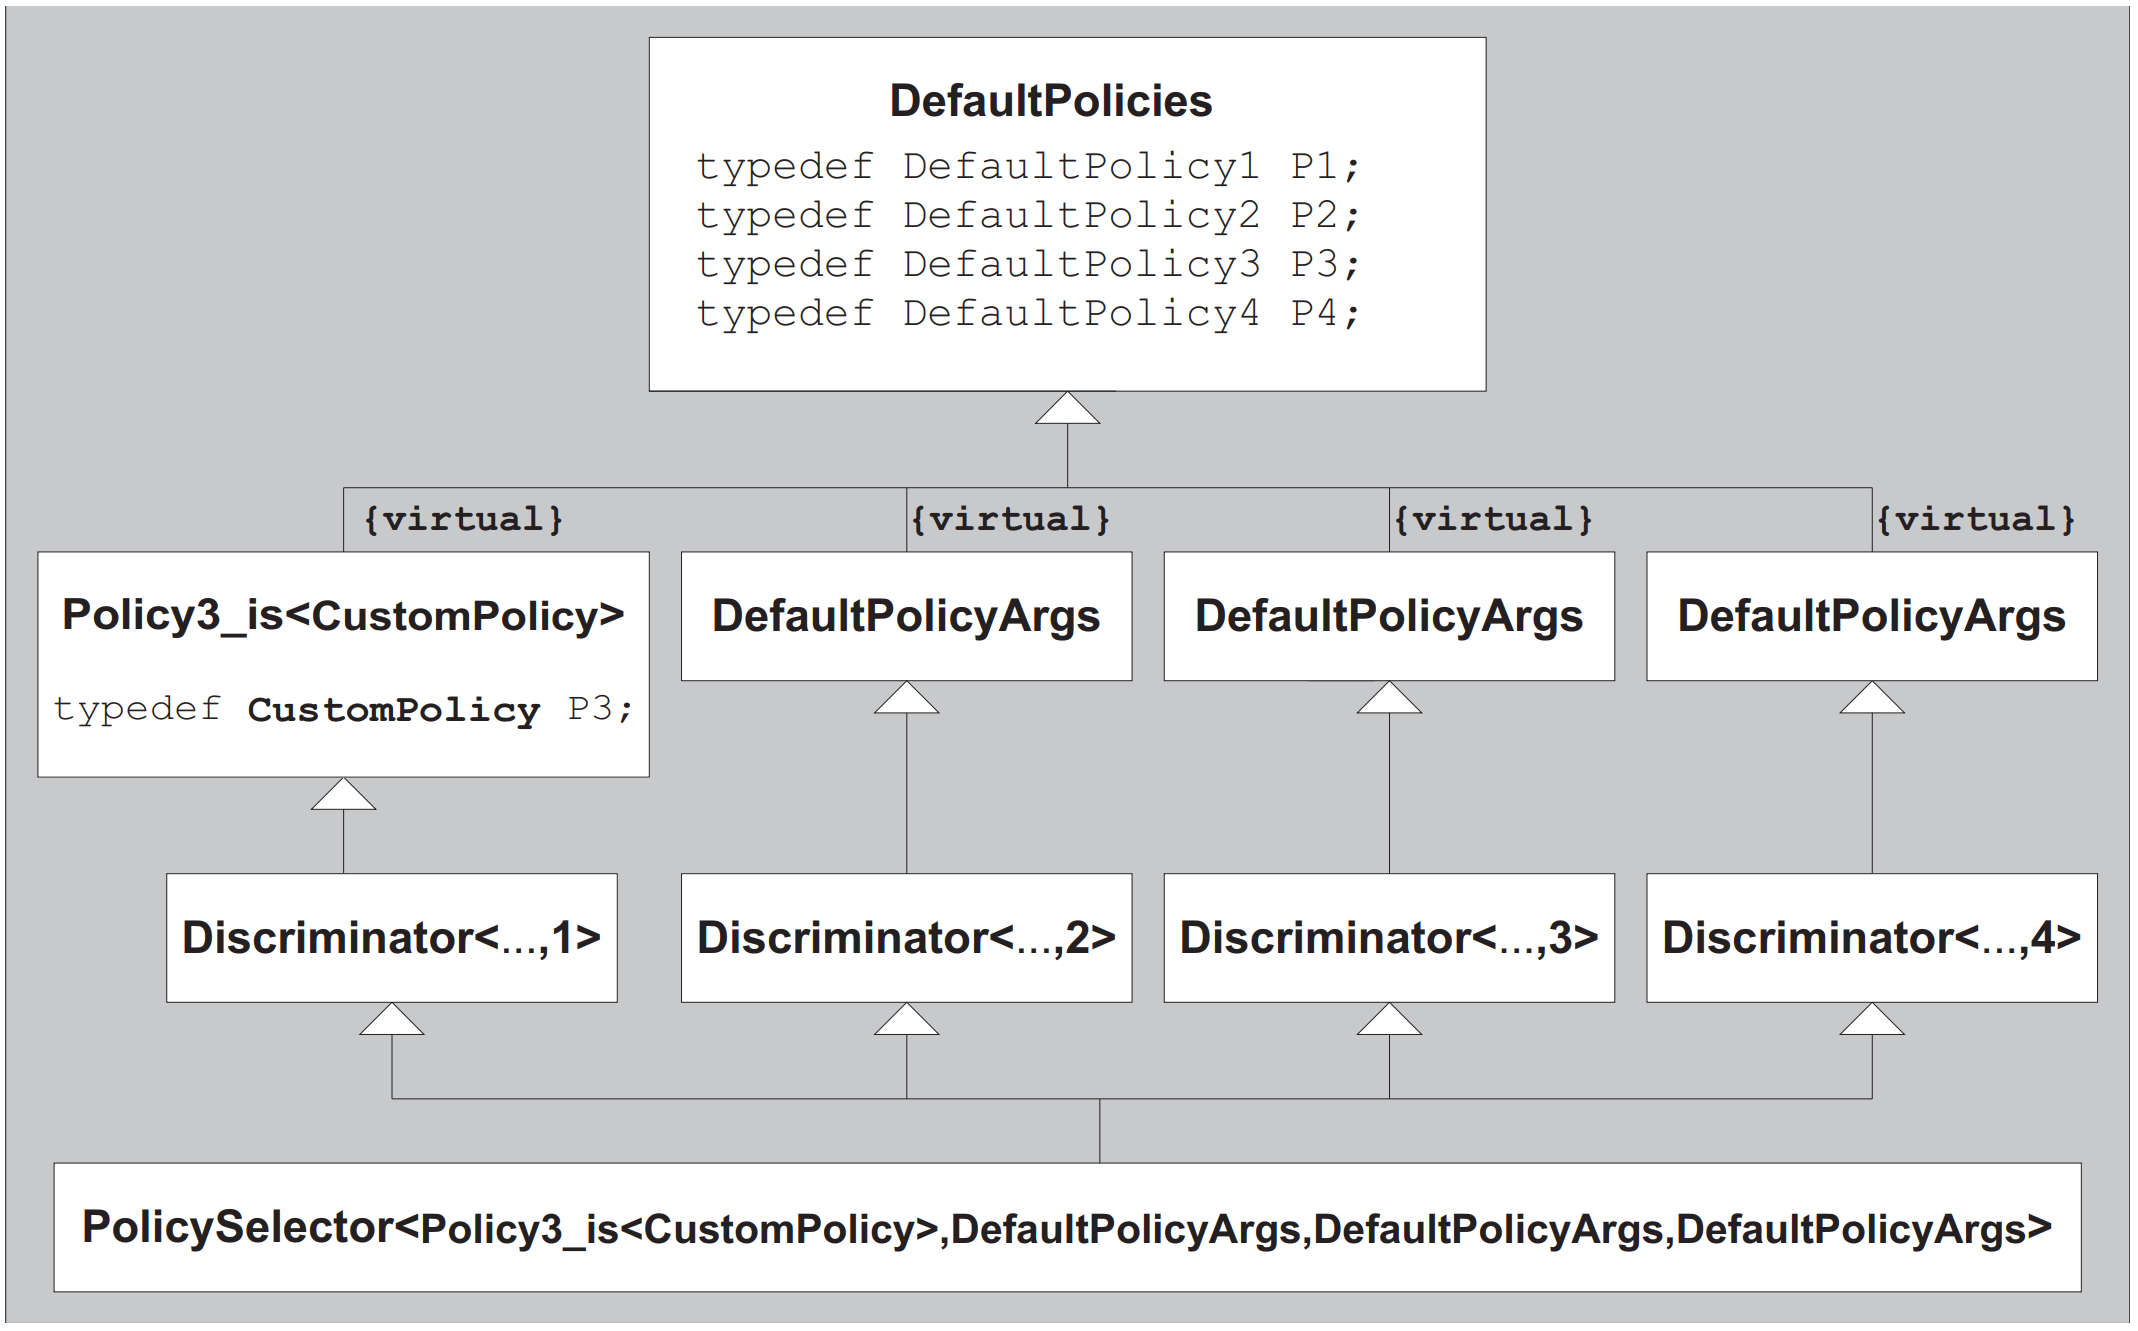
\includegraphics[width=0.8\textwidth]{content/3/chapter21/images/4.png} \\
图21.4. BreadSlicer<>::Policies具有架构的结果类型
\end{center}

都有相同的虚基类DefaultPolicies,定义了P1、P2、P3和P4的默认类型,但P3在一个派生类中重新定义——即在Policy3\_is<>中定义。根据控制规则,这个定义隐藏了基类的定义,因此没有歧义。

\begin{tcolorbox}[colback=webgreen!5!white,colframe=webgreen!75!black]
\hspace*{0.75cm}可以在第一个C++标准的10.2/6节(参见[C++98])中找到控制规则,并在[EllisStroustrupARM]的10.1.1节中对它进行了讨论。
\end{tcolorbox}

在BreadSlicer模板中,可以使用诸如Policies::P3这样的限定名称来引用这四个策略。例如:

\begin{lstlisting}[style=styleCXX]
template<...>
class BreadSlicer {
	...
	public:
	void print () {
		Policies::P3::doPrint();
	}
	...
};
\end{lstlisting}

在inherit/namedtmpl.cpp中可以找到整个示例。

我们开发了用于四个模板类型参数的技术,显然可以扩展到任何合理数量的此类参数,我们从未实例化包含虚基类的辅助类对象。因此,虚基类并不会导致性能或内存消耗的问题。






